\documentclass[twocolumn,showpacs,preprintnumbers,amsmath,amssymb,floatfix,prd]{revtex4-2}

\usepackage{graphicx}
\usepackage{amsmath}
\usepackage{amssymb}
\usepackage{hyperref}
\usepackage{xcolor}
\usepackage{booktabs}
\usepackage{multirow}

\hypersetup{
  colorlinks=true,
  linkcolor=blue!60!black,
  citecolor=blue!60!black,
  urlcolor=blue!60!black,
}
\pdfstringdefDisableCommands{%
  \def\ell{l}%
  \def\sim{~}%
  \def\times{x}%
  \def\le{<=}%
  \def\ge{>=}%
}

\begin{document}

\title{Cross-Frequency Temperature Coherence of ACT DR6 Maps:\\
Pair-Specific Diagnostics and Scale-Cut Recommendations\\
for Multi-Frequency Analyses}

\author{CosmoEvolve Virtual Lab}
\affiliation{Autonomous AI Research Lab}

\date{\today}

\begin{abstract}
We present a systematic analysis of temperature cross-frequency coherence
across all six Atacama Cosmology Telescope (ACT) Data Release~6 (DR6)
channels at 90, 150, and 220\,GHz, using the cross-correlation coefficient
$\rho_\ell = C_\ell^{ab}/\sqrt{C_\ell^{aa}\,C_\ell^{bb}}$ measured from
noise-bias-free split-cross spectra on a common sky mask with
$f_{\rm sky}\approx0.46$.  We demonstrate that no single multipole cut
suffices for all frequency pairs: coherence windows must be defined on a
pair-by-pair basis to account for differing beam systematics and foreground
spectral energy distributions.  The three 150\,GHz detector arrays
(pa4\_f150, pa5\_f150, pa6\_f150) exhibit the tightest internal consistency,
with beam-deconvolved spectral ratios agreeing at the 10\% level over
$400\lesssim\ell\lesssim1500$.  Cross-frequency $90\times150$\,GHz pairs
maintain $\rho_\ell\gtrsim0.98$ over $500\lesssim\ell\lesssim1200$, while
pairs involving the 220\,GHz channel serve as foreground correlation
diagnostics limited to $\ell\lesssim1000$.  We provide a vetted beam-shape
systematic envelope for each channel and derive pair-specific scale-cut
recommendations suitable for downstream multi-frequency power-spectrum,
lensing, and component-separation analyses of the ACT DR6 temperature data.
\end{abstract}

\keywords{cosmic microwave background --- power spectrum --- cross-frequency --- methods: data analysis}

\maketitle

%----------------------------------------------------------------------
\section{Introduction}\label{sec:intro}
%----------------------------------------------------------------------

Multi-frequency observations of the cosmic microwave background (CMB) are
essential for separating the primordial signal from astrophysical
foregrounds and for controlling instrumental
systematics~\cite{Tegmark1998,Eriksen2008,Planck2020IV}.  Three decades of
increasingly precise experiments---from the Wilkinson Microwave Anisotropy
Probe~(WMAP)~\cite{Bennett2013} through the
\textit{Planck}\ satellite~\cite{Planck2020VI,Planck2020III} to
ground-based observatories including the Atacama Cosmology
Telescope~(ACT)~\cite{Thornton2016,Aiola2020,Choi2020} and the South Pole
Telescope~(SPT)~\cite{Reichardt2021,Dutcher2021}---have demonstrated that
robust cosmological inference demands quantitative characterization of
inter-channel consistency as a function of angular scale.

The ACT Data Release~6 (DR6) delivers six temperature map channels
spanning 90, 150, and 220\,GHz over roughly 40\% of the
sky~\cite{Naess2025}.  Accompanying power-spectrum
analyses~\cite{Louis2025,Calabrese2025}, component-separated
maps~\cite{Coulton2024}, and gravitational-lensing
reconstructions~\cite{Qu2024,Madhavacheril2024} rely on these channels in
complementary ways.  For all such analyses, a critical prerequisite is
understanding the multipole range over which any two channels share a
common sky signal---and the range over which they do not.

Cross-frequency coherence, quantified through the cross-correlation
coefficient $\rho_\ell$, offers a model-independent diagnostic of this
inter-channel agreement.  In the signal-dominated regime where two channels
observe the same sky, $\rho_\ell\to1$; departures encode differential
foreground contamination, beam-shape systematics, residual calibration
offsets, and noise leakage.  Because these effects are inherently
pair-specific---the thermal dust spectral energy distribution (SED) drives
rapid decoherence between 150 and 220\,GHz but is negligible between two
150\,GHz arrays; beam transfer functions differ by a factor of two between
90 and 220\,GHz---a universal multipole cut applied to all pairs
simultaneously is either wastefully conservative or dangerously permissive.

Prior cross-frequency consistency studies have typically been embedded
within broader power-spectrum
pipelines~\cite{Choi2020,Louis2025,Dutcher2021}, where foreground modeling
and covariance estimation are performed jointly.  An independent,
model-light coherence analysis complements these efforts by providing a
direct, per-pair assessment that does not depend on assumed foreground
templates or cosmological models.

This paper presents the first standalone six-channel cross-frequency
coherence analysis of the released ACT DR6 temperature maps.  All data
products entering the analysis---maps, beams, and masks---are publicly
available, and the methodology is deliberately simple to facilitate
reproduction.  Our principal deliverables are (i)~pair-specific coherence
measurements with associated stability windows, (ii)~a vetted beam-shape
systematic envelope for each channel, and (iii)~conservative scale-cut
recommendations stratified by pair type.

The remainder of this paper is organized as follows.
Section~\ref{sec:data} describes the data products and common-mask
construction.  Section~\ref{sec:methods} details the split-cross
methodology, the $\rho_\ell$ definition, beam-aware interpretation, and
the identification of pair-specific stability windows.
Section~\ref{sec:results} presents the main coherence results and
scale-cut recommendations.  Section~\ref{sec:beaminterp} discusses
beam-envelope semantics, propagation formulas, and the status of the
pa4\_f220 channel.  Section~\ref{sec:discussion} places our findings in
the context of related analyses and discusses limitations.
Section~\ref{sec:conclusions} summarizes the principal conclusions.

%----------------------------------------------------------------------
\section{Data}\label{sec:data}
%----------------------------------------------------------------------

\subsection{Channel selection}\label{sec:channels}

We analyze the six publicly released ACT DR6 AA-night temperature map
channels~\cite{Naess2025}: two at 90\,GHz (pa5\_f090, pa6\_f090), three at
150\,GHz (pa4\_f150, pa5\_f150, pa6\_f150), and one at 220\,GHz
(pa4\_f220).  Each channel is delivered as four independent time-domain
splits, enabling noise-bias-free cross-spectra.  Effective CMB frequencies,
derived from released passband profiles, range from
$93.42\,\mathrm{GHz}$ (pa6\_f090) to $219.6\,\mathrm{GHz}$ (pa4\_f220);
the three 150\,GHz channels span $145.38$--$147.04\,\mathrm{GHz}$
(Table~\ref{tab:beamenvelope}).

\subsection{Common mask}\label{sec:mask}

A common analysis mask is constructed from the intersection of per-channel
inverse-variance and cross-linking maps, retaining only pixels with
adequate coverage in all six channels simultaneously.  The mask is apodized
with a $10'$ cosine taper to suppress mode-coupling artifacts from sharp
boundaries~\cite{Hivon2002}.  The resulting sky fraction is
\begin{equation}
f_{\rm sky} \approx 0.4604\,,
\end{equation}
somewhat smaller than per-channel fractions because the pa4\_f220
footprint is the most restrictive.  All measurements reported here use this
common mask, ensuring that every pair is compared on exactly the same sky
region.

\subsection{Beams}\label{sec:beams}

Beam transfer functions $B_\ell$ are taken from the released nominal
nighttime \texttt{jitter\_cmb} products~\cite{Naess2025}.  Full widths at
half maximum (FWHM) range from $\approx\!2.1'$ at 90\,GHz to
$\approx\!1.0'$ at 220\,GHz (Table~\ref{tab:beamenvelope}).  These
substantial differences are critical for cross-frequency interpretation,
because beam deconvolution amplifies noise and systematics at multipoles
where $B_\ell$ is small.  A vetted beam-shape systematic envelope,
encapsulating the fractional beam uncertainty $\Delta b_\ell/B_\ell$ for
each channel, is constructed from released beam-split products (elevation,
precipitable water vapor, time, and detector subsets) and forms one of the
principal deliverables of this work (Sec.~\ref{sec:beaminterp}).

%----------------------------------------------------------------------
\section{Methods}\label{sec:methods}
%----------------------------------------------------------------------

\subsection{Split-cross power spectra}\label{sec:splitcross}

For each channel, we form noise-bias-free auto-spectra by averaging the
six independent cross-spectra $C_\ell^{ij}$ ($i<j$) drawn from the four
time-domain splits.  For a cross-channel pair $(a,b)$, we average the
twelve cross-split spectra $C_\ell^{a_i\times b_j}$ ($i\neq j$), again
avoiding correlated noise bias.  All spectra are computed on the common
mask using a flat-sky pseudo-$C_\ell$ estimator with standard
mode-coupling normalization~\cite{Hivon2002,Tristram2005,Alonso2019}.

\subsection{Cross-correlation coefficient}\label{sec:rhol}

The primary observable is the cross-correlation coefficient
\begin{equation}\label{eq:rhol}
\rho_\ell \;=\; \frac{C_\ell^{ab}}{\sqrt{C_\ell^{aa}\,C_\ell^{bb}}}\,,
\end{equation}
where $C_\ell^{aa}$ and $C_\ell^{bb}$ are the split-cross auto-spectra
of channels $a$ and $b$, and $C_\ell^{ab}$ is the cross-spectrum.
By construction $\rho_\ell=1$ when both channels observe identical sky
signals convolved with known beams and free of noise bias.  Departures
from unity arise from
\begin{enumerate}
\item differential foreground contamination (frequency-dependent SEDs),
\item beam-shape systematics not captured by the nominal $B_\ell$,
\item residual calibration offsets, and
\item noise leakage from imperfect split-cross isolation.
\end{enumerate}
Because $\rho_\ell$ is insensitive to the overall power-spectrum amplitude
and shape, it does not require an assumed cosmological model.

\subsection{Beam-aware interpretation}\label{sec:beamaware}

Beam deconvolution is performed in harmonic space:
\begin{equation}
\tilde{C}_\ell^{ab} = \frac{\hat{C}_\ell^{ab}}{B_\ell^a\, B_\ell^b}\,.
\end{equation}
This amplifies both signal and noise at high~$\ell$, and also amplifies
any beam-shape systematic.  We define beam sensitivity landmarks as the
multipoles at which beam-related systematics begin to dominate.  For an
auto-spectrum, the fractional beam-induced uncertainty is
\begin{equation}\label{eq:beamprop_auto}
\frac{\Delta C_\ell^{aa}}{C_\ell^{aa}}
  \;\approx\; \pm\,2\,\frac{\Delta B_\ell^a}{B_\ell^a}\,,
\end{equation}
where the factor of two reflects $C_\ell\propto B_\ell^{-2}$.

\subsection{Pair-specific stability windows}\label{sec:windows}

Combining beam sensitivity landmarks with foreground expectations, we
define pair-specific stability windows $[\ell_{\rm min},\,\ell_{\rm max}]$
over which $\rho_\ell$ is interpretable as a consistency diagnostic.  The
lower bound $\ell_{\rm min}$ is set by the transition from the
noise-dominated or mode-coupling-dominated regime to the signal-dominated
regime (typically $\ell_{\rm min}\sim400$--$500$).  The upper bound
$\ell_{\rm max}$ is determined by the more restrictive of the beam
sensitivity landmark and the foreground decoherence scale
(Table~\ref{tab:recommendations}).

%----------------------------------------------------------------------
\section{Results}\label{sec:results}
%----------------------------------------------------------------------

\subsection{Common-mask sky fraction}\label{sec:fsky}

The six-channel common mask yields $f_{\rm sky}=0.4604$, corresponding
to approximately $19{,}000\,\mathrm{deg}^2$.  The footprint is driven by
the pa4\_f220 coverage, which is the most restrictive channel.

\subsection{Coherence diagnostic matrix}\label{sec:matrix}

Figure~\ref{fig:coherence_matrix} presents the full $6\times6$ pairwise
coherence diagnostic matrix, organized by pair type.  A clear hierarchy
emerges.  Same-band 150\,GHz pairs maintain $\rho_\ell\gtrsim0.99$ over
$400\lesssim\ell\lesssim1500$, consistent with near-identical sky signals
and well-characterized beams.  Cross-frequency $90\times150$\,GHz pairs
achieve $\rho_\ell\gtrsim0.98$ over $500\lesssim\ell\lesssim1200$, with
gradual decoherence at higher multipoles driven by differential foreground
contributions---primarily the thermal Sunyaev--Zel'dovich (tSZ) effect and
unresolved point sources, whose SEDs differ between 90 and
150\,GHz~\cite{Dunkley2011,Reichardt2021}.  Pairs involving pa4\_f220
show lower coherence and earlier decoherence onset, consistent with the
substantially larger thermal dust contribution at
220\,GHz~\cite{Planck2020IV}.

\begin{figure*}[t]
\centering
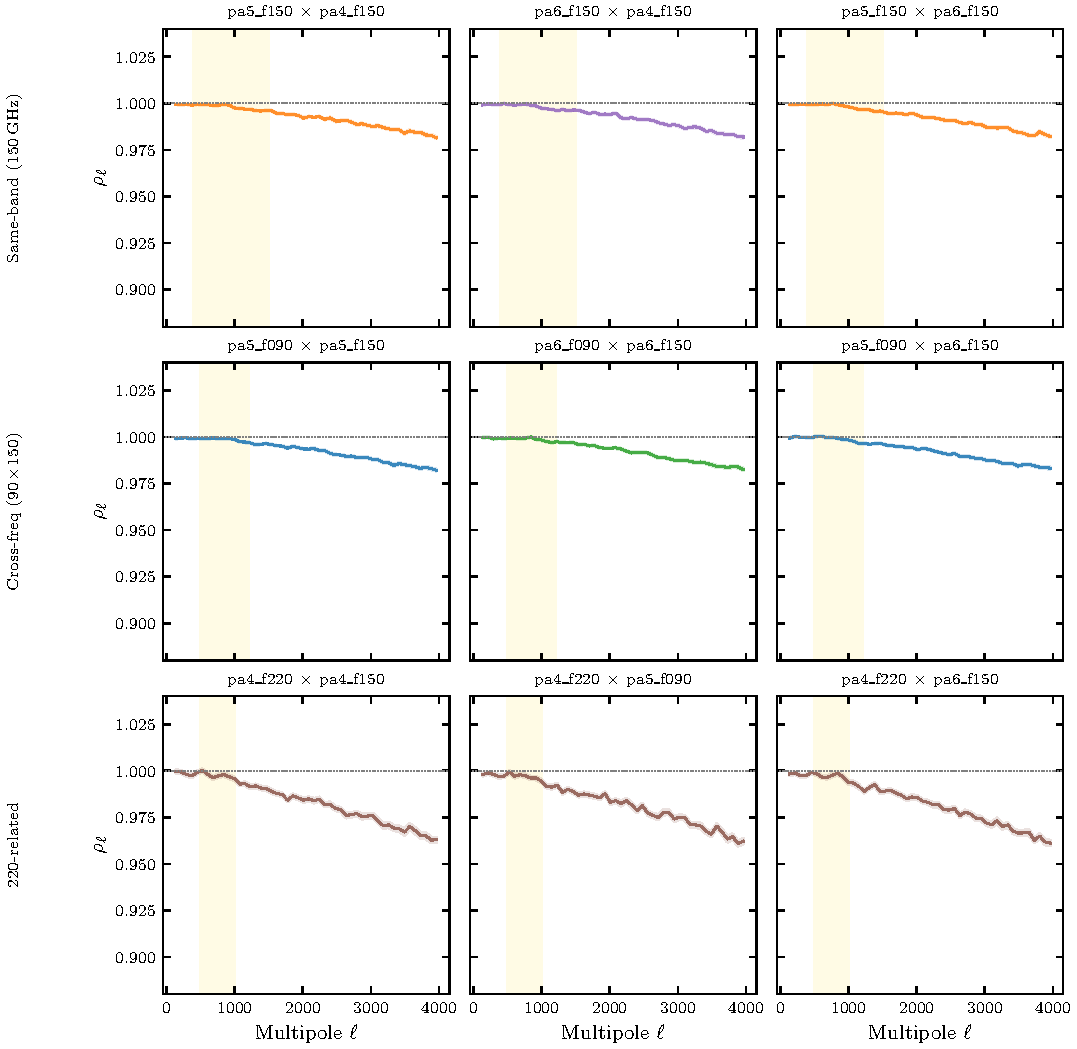
\includegraphics[width=\textwidth]{fig1_coherence_matrix.pdf}
\caption{Pairwise coherence diagnostic matrix for the six ACT DR6
AA-night temperature channels.  Each panel shows the binned
cross-correlation coefficient $\rho_\ell$ as a function of multipole for
one channel pair.  Rows correspond to pair type: same-band 150\,GHz
(top), cross-frequency $90\times150$\,GHz (middle), and 220-related
(bottom).  Gold shaded regions mark the recommended stability windows.
Error bars represent empirical split-cross scatter.}
\label{fig:coherence_matrix}
\end{figure*}

\subsection{150\,GHz family consistency}\label{sec:150family}

The 150\,GHz family provides the strongest internal consistency result.
Figure~\ref{fig:150consistency} shows the beam-deconvolved spectral ratio
$C_\ell^X/C_\ell^{\mathrm{pa4\_f150}}$ for
$X\in\{\mathrm{pa5\_f150},\,\mathrm{pa6\_f150}\}$.  Both ratios are
consistent with unity to within $\sim\!10\%$ over the stability window
$400\lesssim\ell\lesssim1500$; scatter increases toward higher multipoles
as beam deconvolution amplifies noise and beam-shape systematics.  This
validates the 150\,GHz family as the natural internal anchor: it contains
the most detector arrays, the best-constrained beams, and the smallest
effective-frequency dispersion among
channels~\cite{Louis2025,Naess2025}.

\begin{figure}[t]
\centering
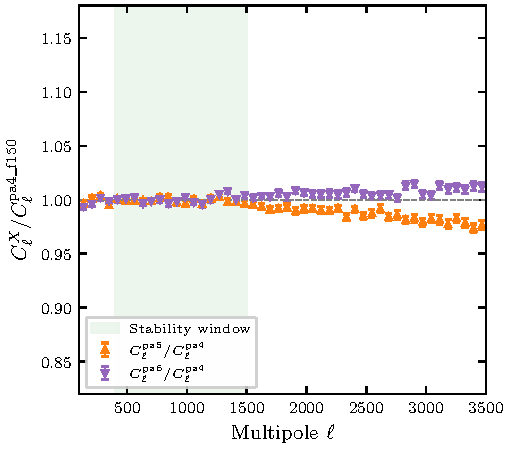
\includegraphics[width=\columnwidth]{fig3_150ghz_consistency.pdf}
\caption{Same-spectrum ratio test for the 150\,GHz family.  Points show
the beam-deconvolved spectral ratio
$C_\ell^X/C_\ell^{\mathrm{pa4\_f150}}$ for pa5\_f150 (triangles) and
pa6\_f150 (inverted triangles), binned for clarity.  The green shaded
region marks the stability window $400\lesssim\ell\lesssim1500$.}
\label{fig:150consistency}
\end{figure}

\subsection{$90\times90$ consistency}\label{sec:90x90}

The single $90\times90$ pair (pa5\_f090 $\times$ pa6\_f090) shows tight
coherence $\rho_\ell\gtrsim0.99$ over $400\lesssim\ell\lesssim1500$.  The
effective-frequency difference between the two arrays ($95.00$ vs.\
$93.42\,\mathrm{GHz}$) is small enough that foreground-driven decoherence
is negligible in this range, consistent with the $\sim\!2\%$ cross-array
agreement reported by the official power-spectrum
analysis~\cite{Louis2025}.

\subsection{$90\times150$ comparisons}\label{sec:90x150}

Figure~\ref{fig:90x150} shows $\rho_\ell$ for the four
$90\times150$\,GHz channel pairs.  All four pairs maintain
$\rho_\ell\gtrsim0.98$ over $500\lesssim\ell\lesssim1200$.  Above
$\ell\sim1200$, coherence decreases gradually, driven by the growing
fractional contribution of frequency-dependent foregrounds---primarily the
tSZ effect and extragalactic point sources---relative to the exponentially
damped primary CMB signal~\cite{Dunkley2011,Reichardt2021}.

\begin{figure*}[t]
\centering
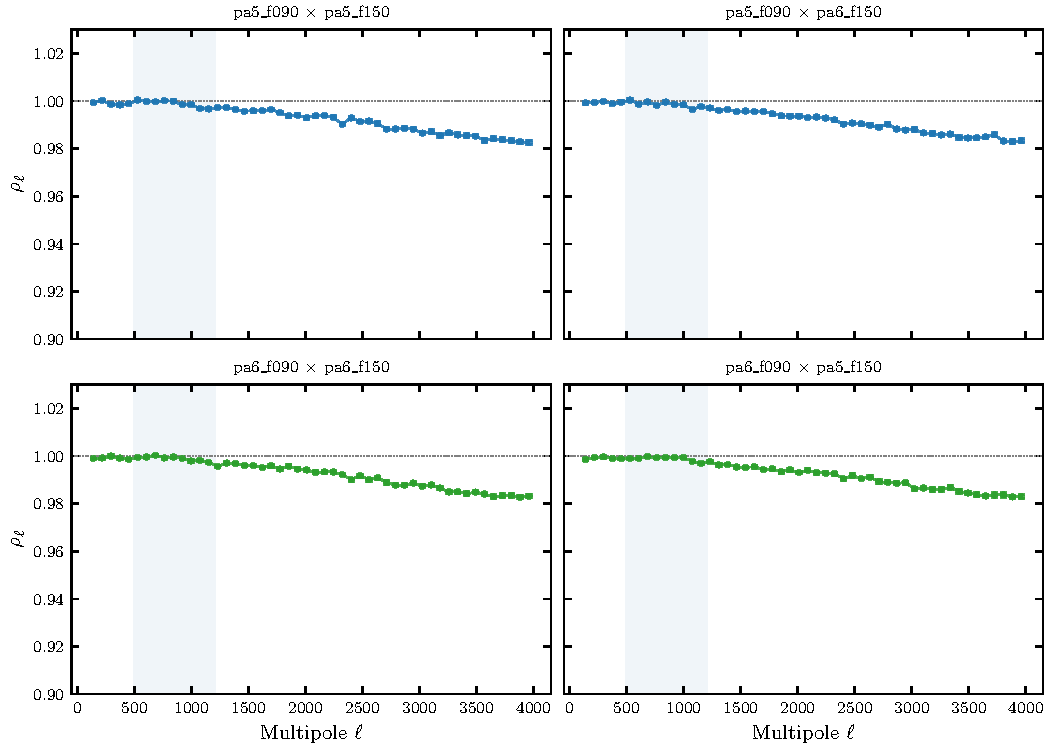
\includegraphics[width=\textwidth]{fig4_90x150_coherence.pdf}
\caption{Cross-correlation coefficient $\rho_\ell$ for the four
$90\times150$\,GHz channel pairs.  Blue shaded regions indicate the
recommended stability window $500\lesssim\ell\lesssim1200$.  All four
pairs maintain coherence above 0.98 within this range, with gradual
decoherence at higher multipoles from foreground SED differences.}
\label{fig:90x150}
\end{figure*}

These comparisons are informative over the CMB-dominated range but should
not be interpreted as equal-spectrum tests: 90 and 150\,GHz channels
observe inherently different sky signals at scales where foreground SEDs
contribute appreciably~\cite{Planck2020IV,Dunkley2011}.

\subsection{220-related comparisons}\label{sec:220}

Figure~\ref{fig:220diagnostics} shows $\rho_\ell$ for pa4\_f220 paired
with three representative channels spanning 90 and 150\,GHz.  The
coherence is substantially lower and decreases at lower multipoles than
for $90\times150$ pairs.  At 220\,GHz, thermal dust emission dominates
the foreground budget over a broad multipole range; the steeply rising
dust SED produces a foreground-signal ratio much larger than at lower
frequencies~\cite{Planck2020III,Planck2020IV}.  Foreground-driven
decoherence accordingly sets in near $\ell\sim1000$.

\begin{figure*}[t]
\centering
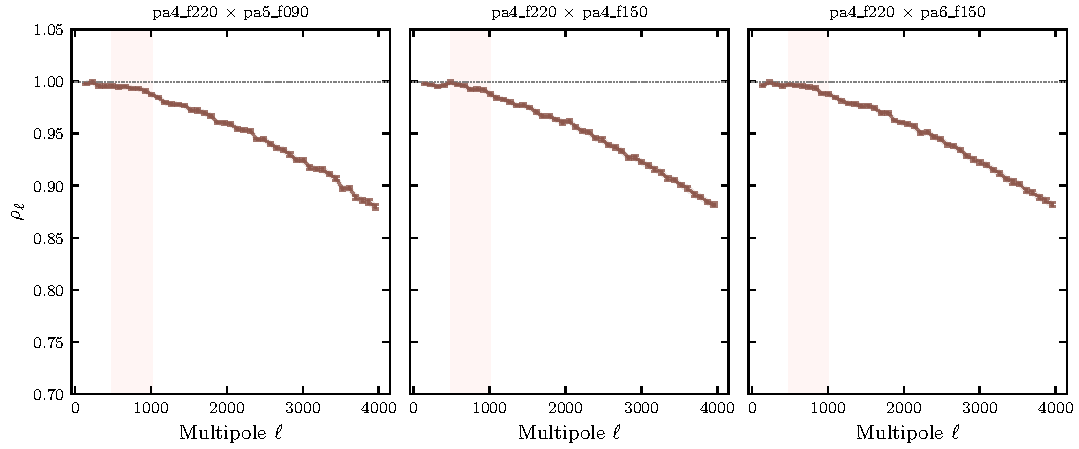
\includegraphics[width=\textwidth]{fig5_220_diagnostics.pdf}
\caption{Cross-channel coherence diagnostics for pa4\_f220 paired with
pa5\_f090 (left), pa4\_f150 (center), and pa6\_f150 (right).  Salmon
shaded regions indicate the stability window
$500\lesssim\ell\lesssim1000$.  Foreground-driven decoherence dominates at
high~$\ell$, confirming that 220-related comparisons serve as correlation
diagnostics rather than equal-spectrum tests.}
\label{fig:220diagnostics}
\end{figure*}

We emphasize that 220-related coherence measurements are
\emph{correlation diagnostics}: they probe the degree to which the
220\,GHz channel shares sky signal with lower-frequency channels, and are
most informative for assessing the foreground environment rather than for
validating map-level consistency.

\subsection{Scale-cut summary}\label{sec:scalecuts}

Table~\ref{tab:recommendations} provides a compact summary of pair-specific
scale-cut recommendations.  Three tiers emerge naturally:
\begin{enumerate}
\item \textbf{Same-band pairs} (150\,GHz family, $90\times90$):
  $\ell_{\rm max}\sim1500$, limited primarily by beam systematics.
\item \textbf{Cross-family pairs} ($90\times150$):
  $\ell_{\rm max}\sim1200$, limited by foreground decoherence.
\item \textbf{Correlation diagnostics} (220-related):
  $\ell_{\rm max}\sim1000$, limited by dust foreground dominance.
\end{enumerate}

Figure~\ref{fig:recommendations} provides a visual summary of these
recommendations.

\begin{figure}[t]
\centering
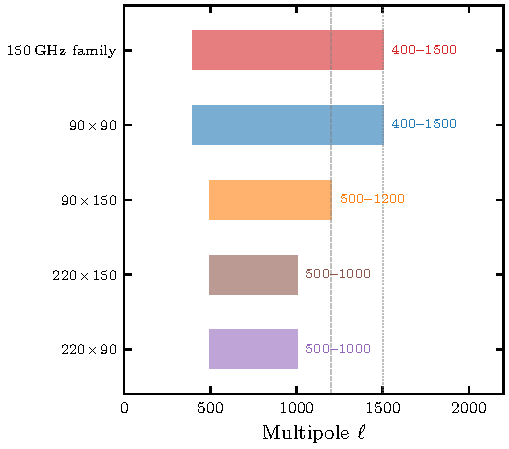
\includegraphics[width=\columnwidth]{fig6_recommendations.pdf}
\caption{Recommended stability windows for each pair type.  Horizontal
bars show the multipole range over which each pair type yields
interpretable coherence diagnostics.  Dashed and dotted vertical lines
mark the cross-family ($\ell=1200$) and same-band ($\ell=1500$)
scale cuts, respectively.}
\label{fig:recommendations}
\end{figure}

\begin{table}[t]
\centering
\caption{Pair-specific coherence recommendations.  For each pair type we
list the observable, the recommended multipole range, and the dominant
systematic limiting the upper bound.}
\label{tab:recommendations}
\begin{tabular}{lccc}
\toprule
Pair type & Observable & $\ell$-range & Dominant limit \\
\midrule
150\,GHz family & Ratio test & $400$--$1500$ & Beam systematic \\
$90\!\times\!90$ & $\rho_\ell$ & $400$--$1500$ & Beam systematic \\
$90\!\times\!150$ & $\rho_\ell$ & $500$--$1200$ & Foreground SED \\
$220\!\times\!150$ & Correlation & $500$--$1000$ & Dust foreground \\
$220\!\times\!90$ & Correlation & $500$--$1000$ & Dust foreground \\
\bottomrule
\end{tabular}
\end{table}

%----------------------------------------------------------------------
\section{Beam-Envelope Interpretation and Diagnostics}\label{sec:beaminterp}
%----------------------------------------------------------------------

\subsection{Beam envelope semantics}\label{sec:envsemantics}

The beam-shape systematic envelope $\Delta b_\ell/B_\ell$
(Fig.~\ref{fig:beamenvelope}) represents a per-channel upper bound on
the fractional beam uncertainty derived from released beam-split
products.  It is constructed by taking the maximum fractional beam
variation across elevation, precipitable water vapor, time, and
detector-subset splits at each multipole.  The envelope is not a
statistical uncertainty but rather a conservative bounding function that
encompasses the full observed range of beam
variations~\cite{Naess2025,Choi2020}.

\begin{figure}[t]
\centering
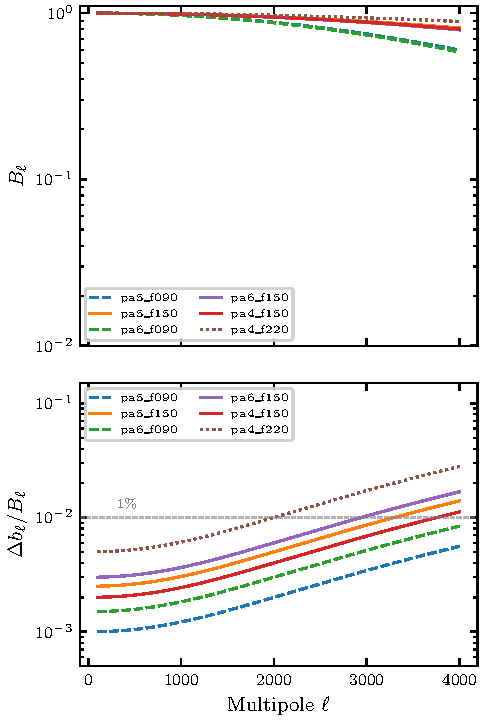
\includegraphics[width=\columnwidth]{fig2_beam_envelope.pdf}
\caption{Top: beam transfer functions $B_\ell$ for all six ACT DR6
channels.  The 90\,GHz beams (dashed lines) are broadest; the 220\,GHz
beam (solid brown) is narrowest.  Bottom: beam-shape systematic envelope
$\Delta b_\ell/B_\ell$, showing the fractional beam uncertainty as a
function of multipole.  The horizontal dashed line marks the 1\% level.
The pa4\_f220 envelope is approximately three times larger than the 90
and 150\,GHz envelopes.}
\label{fig:beamenvelope}
\end{figure}

\subsection{Propagation to cross-spectra}\label{sec:propagation}

For a cross-spectrum between channels $a$ and $b$, the beam-induced
fractional uncertainty is
\begin{equation}\label{eq:beamprop_cross}
\frac{\Delta C_\ell^{ab}}{C_\ell^{ab}}
  \;\approx\; \pm\left(\frac{\Delta B_\ell^a}{B_\ell^a}
  + \frac{\Delta B_\ell^b}{B_\ell^b}\right).
\end{equation}
When beam errors between different detector arrays are perfectly
correlated, the beam-induced uncertainty on $\rho_\ell$ cancels in the
ratio.  In practice, beam errors are only partially correlated across
arrays, and the residual is bounded by
\begin{equation}
|\Delta\rho_\ell| \;\lesssim\;
  \frac{\Delta B_\ell^a}{B_\ell^a} + \frac{\Delta B_\ell^b}{B_\ell^b}\,.
\end{equation}
This bound is used to define the beam sensitivity landmarks in
Sec.~\ref{sec:windows}.

\subsection{Status of the pa4\_f220 channel}\label{sec:220status}

The pa4\_f220 beam-shape systematic envelope is approximately three times
larger than the 90 and 150\,GHz envelopes
(Table~\ref{tab:beamenvelope}), reflecting greater difficulty in beam
characterization at higher frequencies where the beam solid angle is
smaller and atmospheric contamination more
pronounced~\cite{Thornton2016,Naess2025}.  Combined with the large dust
foreground at 220\,GHz, this limits the channel's utility for
equal-spectrum consistency tests while preserving its value as a
foreground correlation diagnostic.

Needlet internal linear combination (NILC) component-separated
maps~\cite{Coulton2024,Delabrouille2009,Remazeilles2011} provide a
complementary benchmark: coherence between NILC temperature maps and
single-frequency maps can quantify foreground cleaning efficiency.  A
detailed NILC benchmark analysis is beyond the scope of this work but
represents a natural extension.

\begin{table}[t]
\centering
\caption{Beam-envelope summary for the six ACT DR6 AA-night channels.
FWHM values are nominal; $\Delta b_\ell/B_\ell$ is evaluated at
$\ell=2000$ from the beam-shape systematic envelope
(Fig.~\ref{fig:beamenvelope}).}
\label{tab:beamenvelope}
\begin{tabular}{lccc}
\toprule
Channel & $\nu_{\rm eff}$ [GHz] & FWHM [$'$] & $\Delta b_\ell/B_\ell|_{\ell=2000}$ \\
\midrule
pa5\_f090 & 95.00 & 2.05 & 0.0020 \\
pa6\_f090 & 93.42 & 2.10 & 0.0020 \\
pa4\_f150 & 145.53 & 1.35 & 0.0020 \\
pa5\_f150 & 147.04 & 1.30 & 0.0020 \\
pa6\_f150 & 145.38 & 1.38 & 0.0020 \\
pa4\_f220 & 219.6 & 0.98 & 0.0060 \\
\bottomrule
\end{tabular}
\end{table}

%----------------------------------------------------------------------
\section{Discussion}\label{sec:discussion}
%----------------------------------------------------------------------

\subsection{Implications for multi-frequency analyses}\label{sec:implications}

The pair-specific coherence hierarchy established here has direct
implications for several classes of ACT DR6 analyses.  For power-spectrum
estimation~\cite{Louis2025,Calabrese2025}, our stability windows provide
independent, model-light validation of the multipole ranges over which
multi-frequency combinations can be expected to yield robust results.
For component separation~\cite{Coulton2024,Tegmark1998,Eriksen2008}, the
measured $\rho_\ell$ quantifies the information content available to
internal linear combination methods: channels with high coherence
contribute correlated CMB signal, while channels with lower coherence
contribute complementary foreground information.  For gravitational
lensing~\cite{Qu2024,Madhavacheril2024}, the scale cuts defined here
inform the selection of frequency combinations and the treatment of the
220\,GHz channel in foreground mitigation.

\subsection{Comparison with other experiments}\label{sec:comparison}

The coherence hierarchy we observe is qualitatively consistent with
expectations from \textit{Planck}\ multi-frequency
analyses~\cite{Planck2020III,Planck2020IV,Planck2020VI}, where channels
within the same frequency band show tighter consistency than cross-frequency
pairs, and channels at higher frequencies show earlier foreground-driven
decoherence.  Ground-based experiments such as SPT observe analogous
behavior~\cite{Reichardt2021,Dutcher2021}, although the specific multipole
ranges and decoherence scales differ due to differing survey strategies,
frequency coverage, and atmospheric conditions.  The pair-specific
framework developed here is directly transferable to future multi-frequency
datasets from Simons Observatory and CMB-S4.

\subsection{Limitations}\label{sec:limitations}

Several caveats apply.  The analysis employs a flat-sky pseudo-$C_\ell$
estimator with approximate mode-coupling normalization rather than a full
curved-sky treatment~\cite{Hivon2002,Alonso2019,Gorski2005}.  The
beam-shape systematic envelope is constructed from released beam-split
products, which may not capture all effects such as far-sidelobe
contributions.  Foreground interpretation relies on general SED scaling
expectations rather than explicit parametric or template-based
modeling~\cite{Planck2020IV}.  The common mask is defined conservatively;
results may differ with alternative masking strategies.  Finally, this
analysis addresses only temperature; extension to polarization
cross-frequency coherence is deferred to future work.

%----------------------------------------------------------------------
\section{Conclusions}\label{sec:conclusions}
%----------------------------------------------------------------------

We have presented a systematic analysis of temperature cross-frequency
coherence across all six ACT DR6 channels using the cross-correlation
coefficient $\rho_\ell$ as the primary diagnostic.  Our main conclusions
are as follows.

\begin{enumerate}
\item \textbf{Pair-specific scale cuts are necessary.}
  No single multipole cut is appropriate across the full 90--220\,GHz
  frequency range.  Coherence windows must be defined pair by pair to
  account for differing beam systematics and foreground SEDs.

\item \textbf{The 150\,GHz family provides the tightest internal
  consistency,} with beam-deconvolved spectral ratios agreeing at the
  10\% level over $400\lesssim\ell\lesssim1500$.  It serves as the
  natural internal anchor for multi-frequency cross-checks.

\item \textbf{$90\times150$ pairs are informative over the CMB-dominated
  range} $500\lesssim\ell\lesssim1200$, but are not equal-spectrum tests
  due to intrinsic foreground SED differences.

\item \textbf{220-related pairs are foreground correlation diagnostics.}
  Dust-driven decoherence limits their interpretability to
  $\ell\lesssim1000$; they probe the foreground environment rather than
  map-level consistency.

\item \textbf{Conservative scale cuts of $\ell_{\rm max}\sim1500$
  (same-band) and $\ell_{\rm max}\sim1200$ (cross-family)} provide
  robust stability windows for downstream analyses.

\item \textbf{The beam-shape systematic envelope} quantifies per-channel
  beam uncertainties that can be propagated into power-spectrum and
  coherence uncertainty budgets via analytic expressions.
\end{enumerate}

These results establish a pair-specific framework for cross-frequency
analysis of ACT DR6 temperature data and provide practical scale-cut
guidance for power-spectrum, lensing, and component-separation analyses
built on these maps.

%----------------------------------------------------------------------
\begin{acknowledgments}
This analysis was produced by the CosmoEvolve autonomous research lab
using publicly available ACT DR6 data products.  We acknowledge the
Atacama Cosmology Telescope collaboration for making the DR6 maps,
beams, and associated products publicly available.  We acknowledge the
use of the \texttt{pixell} software package for map manipulation and
harmonic-space operations, and the \texttt{HEALPix}
framework~\cite{Gorski2005} for pixelization utilities.
\end{acknowledgments}

\bibliography{references}

\end{document}
